%   MSc Business Analytics Dissertation
%   Format based on skeleton template provided as part of module MIS40750
%
%   Title:     Optimising the design of buffer preparation in bioprocessing
%              facilities
%   Author:    Sean Tully
%
%   Chapter 5: Results
%
%   Change Control:
%   When     Who   Ver  What
%   -------  ----  ---  --------------------------------------------------------
%   06Jun16  ST    0.1  Begun 
%

\chapter{Results}\label{C.results}

\begin{quote}
Bosh! Stephen said rudely.
A man of genius makes no mistakes.
His errors are volitional and are the portals of discovery.

\hspace{2cm}--- James Joyce, \emph{Ulysses}
\end{quote}

\section{Introduction}\label{S.intro5}
\begin{figure}
    \centering
    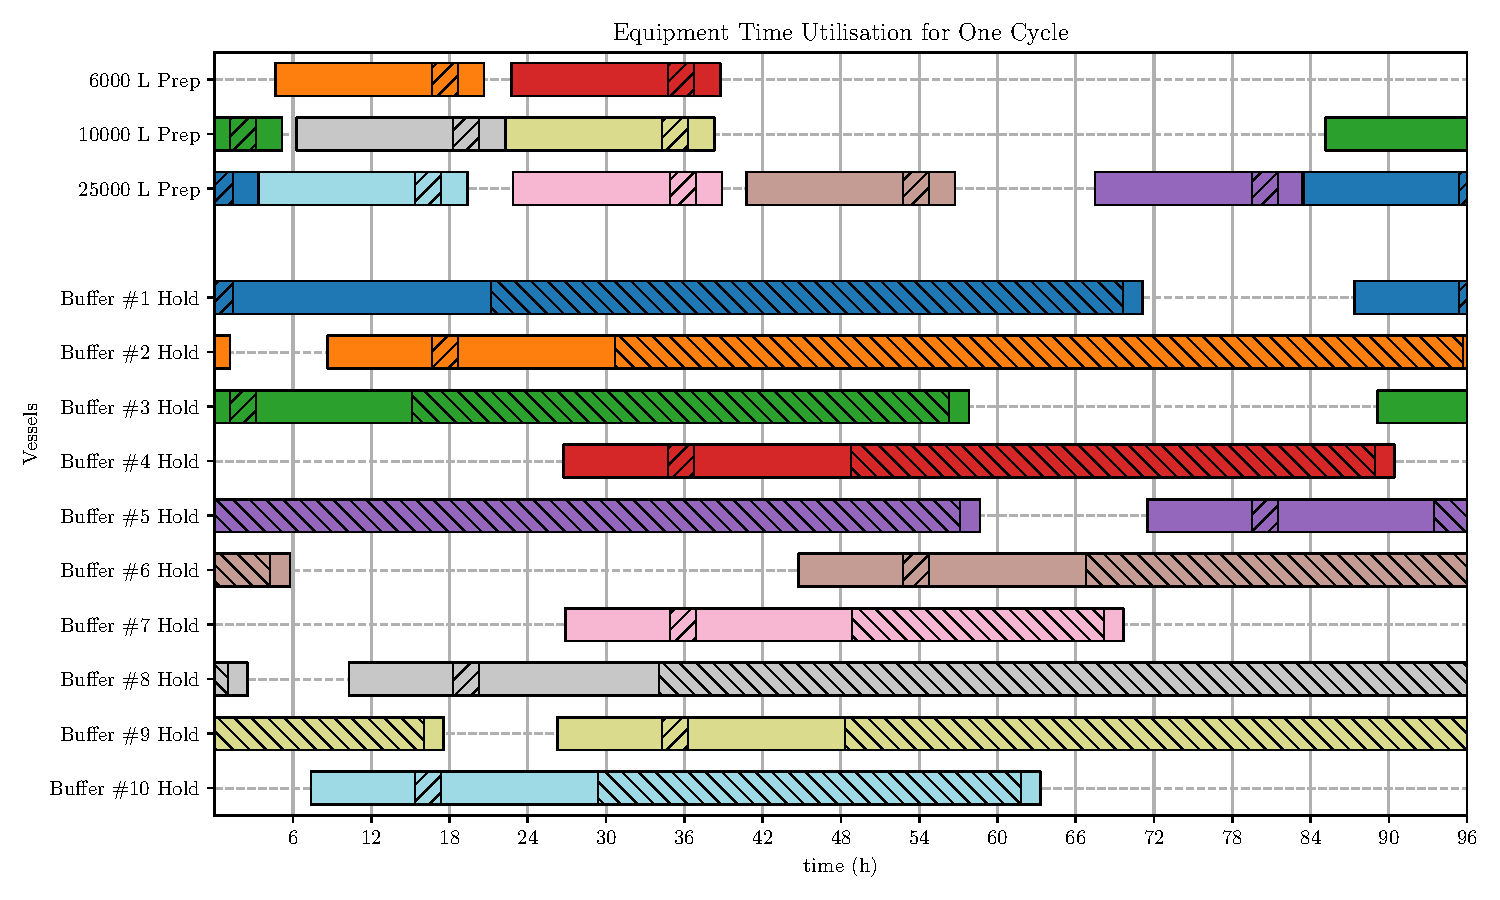
\includegraphics[angle=0,scale=0.55]{../examples/large-scale/plot2.pdf}
    \caption{Equipment time utilisation for large-scale example}
    \label{fig.etu}
\end{figure}
The equipment time utilisation plot for the sample data given in 
\hyperref[C.data]{Chapter \ref*{C.data}} is given in
\hyperref[fig.etu]{Figure \ref*{fig.etu}}.

%TODO
\textbf{TODO: discuss results}

%TODO
\textbf{TODO: generate more datasets}

\section{Complexity}\label{S.complexity}
\begin{figure}
    \centering
    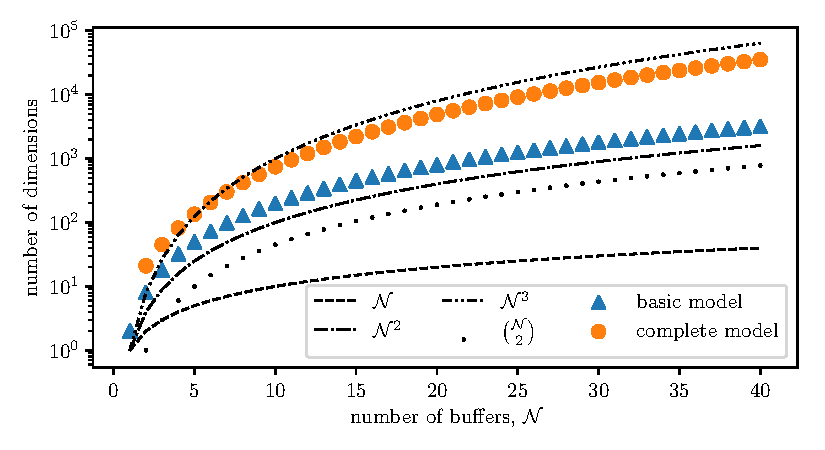
\includegraphics{./figures/dimensions.pdf}
    \caption{Model complexity -- dimensions}
    \label{fig.dims}
\end{figure}
\begin{figure}
    \centering
    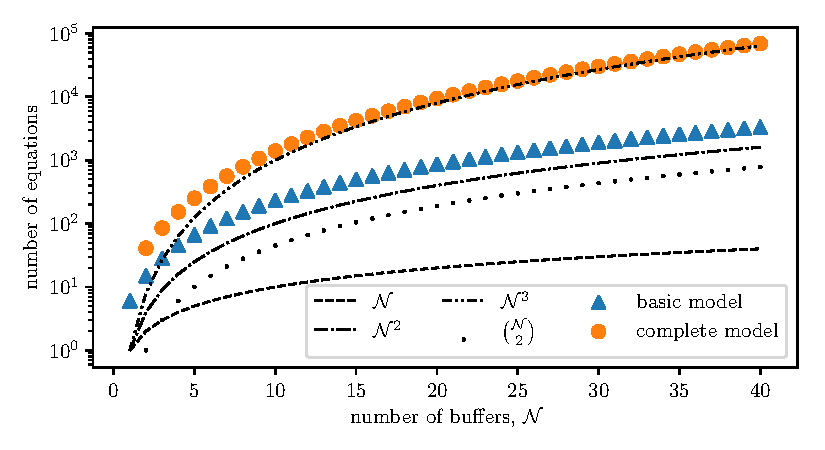
\includegraphics{./figures/equations.pdf}
    \caption{Model complexity -- equations}
    \label{fig.eqns}
\end{figure}

%TODO
\textbf{TODO: recalculate complexities in light of model changes}

The notation for complexity in this section is according to \citet{Knuth:1976}.

Noting that there is a weak dependence on $\mathcal{M}$ and that as the problem
grows larger in terms of $\mathcal{N}$, it is likely that $\mathcal{M}$ will
reach a maximum value, the approximation $\mathcal{M} \approx \mathcal{N}$ may
be used as a conservative simplification when considering complexity.
\begin{table}[h!]
    \centering
    \caption{Model complexity}
    \label{tbl.complexity1}
    \begin{tabular}{l | c | c}
        model & no. of dimensions & no. of equations\\ \hline
        basic & $\mathcal{N}^2 + \mathcal{N} \mathcal{M}$
            & $2\mathcal{N}^2 + 3\mathcal{N} + 1$\\
        complete & $\mathcal{N} {{\mathcal{N}}\choose{2}}
            + 2\mathcal{N}^2 + 2\mathcal{N} +\mathcal{N} \mathcal{M}$
            & $3\mathcal{N} + 7{{\mathcal{N}}\choose{2}} + 6\mathcal{N} + 1$\\
    \end{tabular}
\end{table}
\begin{table}[h!]
    \centering
    \caption{Simplified model complexity}
    \label{tbl.complexity2}
    \begin{tabular}{l | c | c}
        model & no. of dimensions & no. of equations\\ \hline
        basic & $2\mathcal{N}^2$ & $2\mathcal{N}^2 + 3\mathcal{N} + 1$\\
        complete & $\mathcal{N} {{\mathcal{N}}\choose{2}}
            + 2\mathcal{N}^2 + 2{{\mathcal{N}}\choose{2}} + 2\mathcal{N}$
            & $3\mathcal{N} + 7{{\mathcal{N}}\choose{2}} + 6\mathcal{N} + 1$\\
    \end{tabular}
\end{table}
For the simple model, we can see that both the number of dimensions and the
number of equations is $\Theta \left( \mathcal{N}^2 \right)$.

Note that ${{\mathcal{N}}\choose{2}}$ is $\Theta \left( \mathcal{N}^2 \right)$.
Accordingly, for the complete model, the number of dimensions is 
$\Theta \left( \mathcal{N}^3 \right)$ and the number of equations is
$\Theta \left( \mathcal{N}^2 \right)$.

%TODO
\textbf{TODO: time taken as a function of input size and as a function of 
    solver choice}
\begin{figure}
    \centering
    \includegraphics{./figures/timing.pdf}
    \caption{Solution time as a function of buffer count}
    \label{fig.timing}
\end{figure}
    
    
%TODO
\textbf{TODO: boxplots of time taken as a function of input size}
